\section{Derivations}


\subsection{Mean and covariance of integral of Brownian motion}
\label{app:intBM}
Shifted Brownian motion is defined as a Gaussian process $\nu(t)$ on $t \geq 0$, with mean and covariance functions defined as
\be
	m^{(\nu)}(t) = \nu_0
	\quad,\qquad 
	K^{(\nu)}(t, t') = D\,\text{min}(t, t')\quad,
\ee
where $\nu_0$ is the starting point at $t = 0$, and $D$ is the diffusion coefficient of the Brownian motion.

We define the integral of the Brownian motion as the process $\mu(t) = \mu_0 + \intop_0^t \d{x} \nu(x)$ on $t \geq 0$, with mean and covariance functions defined as
\be
	m^{(\mu)}(t) = \mu_0 + \intop_0^{t} \d{x} m^{(\nu)}(x) = \mu_0 + \nu_0 t
	\quad,\qquad
	K^{(\mu)}(t, t') = \intop_0^t \d{x} \intop_0^{t'} \d{y} K^{(\nu)}(x, y)
\ee
The double integral can be separated into 3 non-overlapping parts. With the notation $l = \text{min}(t, t')$ and $h = \text{max}(t, t')$, we can write 
\be
	K^{(\mu)}(t, t') = D\intop_0^h \d{x} \intop_0^{l} \d{y} \text{min}(x, y)
\ee
since $K^{(\nu)}(x,y) = D\,\text{min}(x,y)$ is symmetric in its arguments. The integration domain can be partitioned into three non-overlapping domains,
\begin{figure}[h]
\centering
	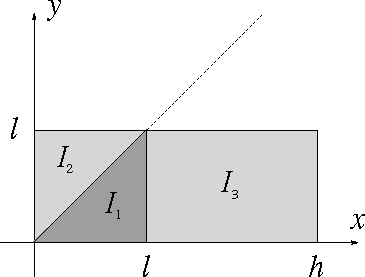
\includegraphics[width=0.3\textwidth]{figs/I1I2I3_regions.pdf}
\end{figure}
\ba
	I_1 &=& \intop_0^l \d{x} \intop_0^x \d{y} \underbrace{\text{min}(x,y)}_{y} \;=\; \intop_0^l \d{x} \frac{x^2}{2} \;=\; \frac{l^3}{6}
	\\
	I_2 &=& \intop_0^l \d{y} \intop_0^y \d{x} \underbrace{\text{min}(x,y)}_{x} \;=\; \intop_0^l \d{y} \frac{y^2}{2} \;=\; \frac{l^3}{6}
	\\
	I_3 &=& \intop_l^h \d{x} \intop_0^l \d{y} \underbrace{\text{min}(x,y)}_{y} \;=\; \intop_l^h \d{x} \frac{l^2}{2} \;=\; (h-l)\frac{l^2}{2}
\ea
the sum of which yields
\be
	K^{(\mu)}(t, t') = D(I_1 + I_2 + I_3) = D\,\frac{l^2}{2}\left(h - \frac{l}{3}\right)  = D\,\frac{\text{min}(t, t')^2}{2}\left(\text{max}(t, t') - \frac{\text{min}(t, t')}{3}\right)
\ee

\subsection{Gaussian integral}
\label{app:gaussian_integral}
Here we calculate the following multi-dimensional Gaussian integral, where $z, \mathcal{B} \in \mathds{R}^n$, $\mathcal{A}\in \mathds{R}^{n\times n}$ (positive definite) and $\mathcal{C} \in \mathds{R}$, 
\ba
	I &:=& \int\d{z} \exp\left(-\frac{1}{2}z\T \mathcal{A} z + \mathcal{B}\T z + \mathcal{C}\right) \\
	&= &
	\int\d{z} \exp\left(-\frac{1}{2}z\T \mathcal{A} z + \frac{1}{2}z\T \mathcal{B} + \frac{1}{2}\mathcal{B}\T z + \mathcal{C}\right) \\
	&=&
	\int\d{z} \exp\left(-\frac{1}{2}\Big(z - \mathcal{A}^{-1}\mathcal{B}\Big)\T \mathcal{A} \Big(z - \mathcal{A}^{-1}\mathcal{B}\Big) + \frac{1}{2}\mathcal{B}\T\mathcal{A}^{-1}\mathcal{B} + \mathcal{C}\right)\\
	&=&
	\exp\left(\frac{1}{2}\mathcal{B}\T\mathcal{A}^{-1}\mathcal{B} + \mathcal{C}\right) \int\d{z'} \exp\left(-\frac{1}{2}(z')\T \mathcal{A} z'\Big)\right).
\ea
Since $\mathcal{A}$ is positive definite there exists an orthogonal matrix $\mathcal{O}$ that diagonalizes it, 
\be
	\mathcal{OAO}\T = \Lambda = \text{diag}(\lambda_1, \lambda_2, \ldots \lambda_n)
\ee
where $\lambda_i$ are the eigenvalues of $\mathcal{A}$. In terms of the transformed coordinates $z'' = \mathcal{O}z'$ we get a separable integral:
\be
	\int\d{z'} \exp\left(-\frac{1}{2}(z')\T \mathcal{A} z'\Big)\right) = \int\d{z''} \exp\left(-\frac{1}{2}(z'')\T \Lambda z''\Big)\right) = \prod_{i=1}^n \int\d{x_i} \exp\left(-\frac{1}{2}x_i \lambda_i x_i\Big)\right)
\ee
Each factor can be simplified using the result for a 1-dimensional Gaussian integral $\int\d{x}\exp(-\frac{1}{2}ax^2) = \sqrt{2\pi / a}$, giving
\be
	\prod_{i=1}^n \sqrt{2\pi / \lambda_i} = \sqrt{\frac{(2\pi)^n}{\prod_i \lambda_i}} = \sqrt{\frac{(2\pi)^n}{\text{det}(\Lambda)}} = \sqrt{\frac{(2\pi)^n}{\text{det}(\mathcal{A})}},
\ee
where $\det{(\Lambda)} = \det{(\mathcal{A})}$, because the transformation matrix $\mathcal{O}$ is orthogonal, i.e. $\det\mathcal{(O)} = 1$. This results in
\be
	I = \exp\left(\frac{1}{2}\mathcal{B}\T\mathcal{A}^{-1}\mathcal{B} + \mathcal{C}\right)\times \sqrt{\frac{(2\pi)^n}{\text{det}(\mathcal{A})}}\quad.
\ee

\section{Implementation}

\subsection{Stan code for \refeq{eq:L}}
